\documentclass{tikzposter} %Options for format can be included here

\usepackage{todonotes}

\usepackage[tikz]{bclogo}
\usepackage{lipsum}
\usepackage{amsmath}

\usepackage{booktabs}
\usepackage{longtable}
\usepackage[absolute]{textpos}
\usepackage[it]{subfigure}
\usepackage{graphicx}
\usepackage{cmbright}
%\usepackage[default]{cantarell}
%\usepackage{avant}
%\usepackage[math]{iwona}
\usepackage[math]{kurier}
\usepackage[T1]{fontenc}


%% add your packages here
\usepackage{hyperref}
% for random text
\usepackage{lipsum}
\usepackage[english]{babel}
\usepackage[pangram]{blindtext}

\colorlet{backgroundcolor}{blue!10}

 % Title, Author, Institute
\title{FLIP01 Final-term Presentation}
\author{Jiahui Zhou$^1$}
\institute{$^1$ Xi'an Shiyou University, China}
%\titlegraphic{logos/tulip-logo.eps}

%Choose Layout
\usetheme{Wave}

%\definebackgroundstyle{samplebackgroundstyle}{
%\draw[inner sep=0pt, line width=0pt, color=red, fill=backgroundcolor!30!black]
%(bottomleft) rectangle (topright);
%}
%
%\colorlet{backgroundcolor}{blue!10}

\begin{document}


\colorlet{blocktitlebgcolor}{blue!23}

 % Title block with title, author, logo, etc.
\maketitle

\begin{columns}
 % FIRST column
\column{0.5}% Width set relative to text width

%%%%%%%%%% -------------------------------------------------------------------- %%%%%%%%%%
 %\block{Main Objectives}{
%  	      	\begin{enumerate}
%  	      	\item Formalise research problem by extending \emph{outlying aspects mining}
%  	      	\item Proposed \emph{GOAM} algorithm is to solve research problem
%  	      	\item Utilise pruning strategies to reduce time complexity
%  	      	\end{enumerate}
%%  	      \end{minipage}
%}
%%%%%%%%%% -------------------------------------------------------------------- %%%%%%%%%%


%%%%%%%%%% -------------------------------------------------------------------- %%%%%%%%%%
\block{Introduction}{
    The competation \textit{Google QUEST Q\&A Labeling} is designed to 
    improving automated understanding of complex question answer content.
    The challenge is to use this new dataset to build predictive algorithms for different subjective aspects of question-answering. 
    The question-answer pairs were gathered from nearly 70 different websites, in a "common-sense" fashion.
    \begin{center}
        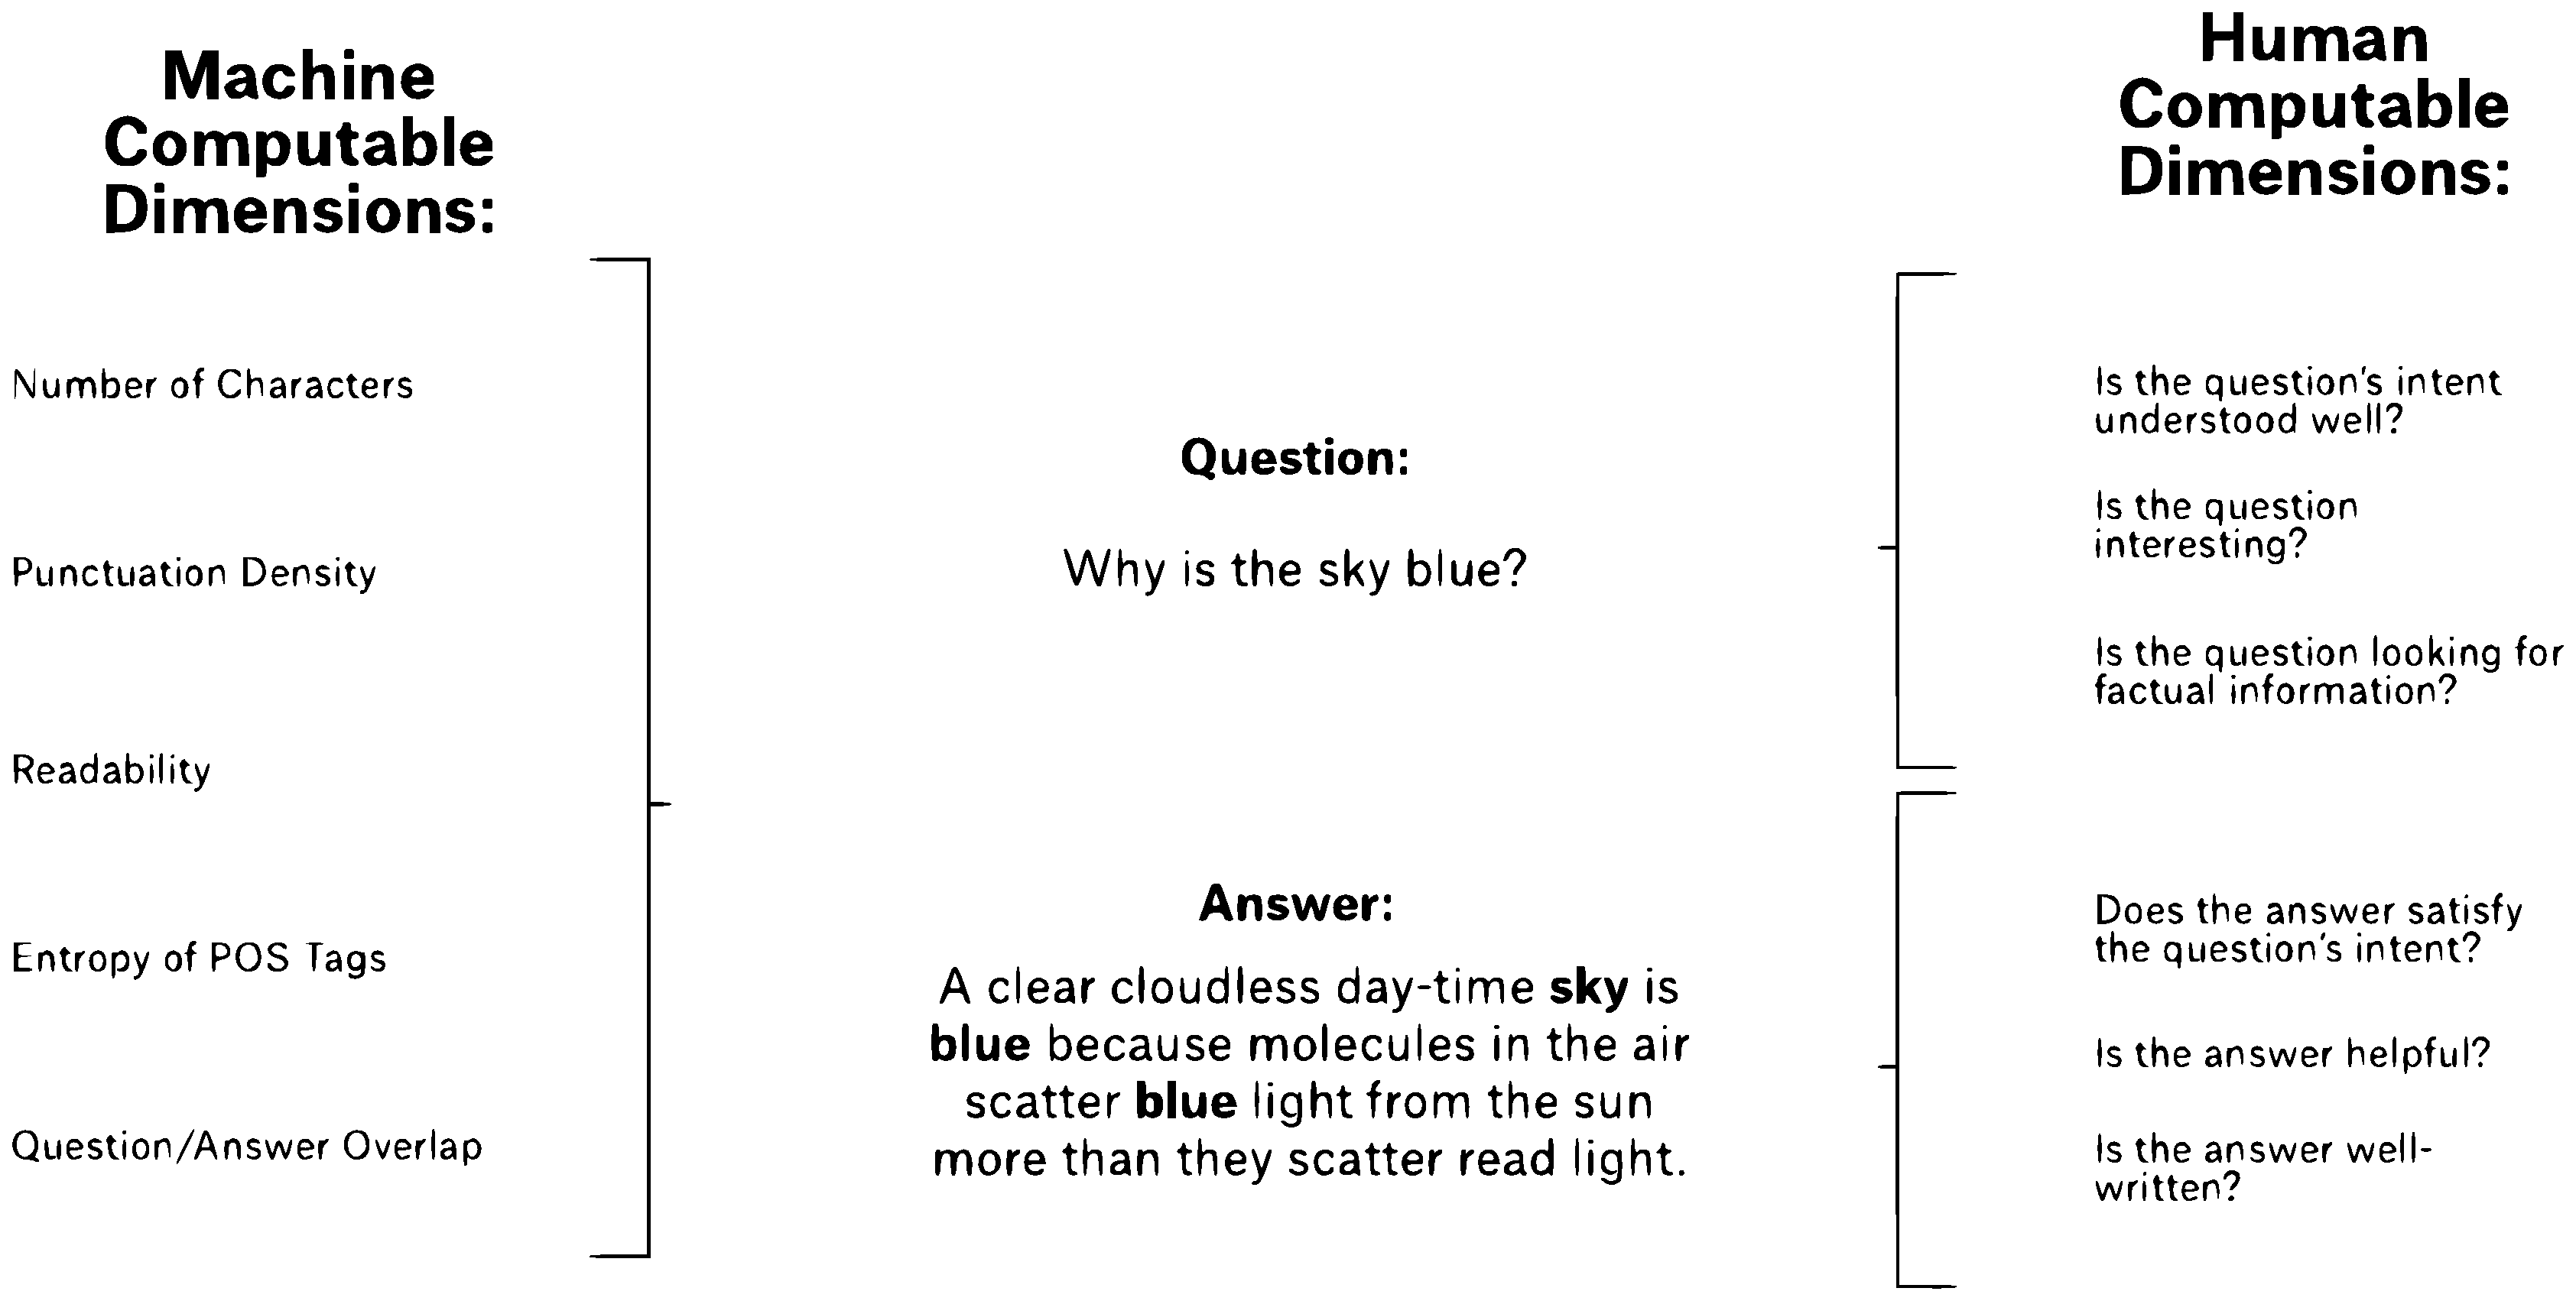
\includegraphics[width=\linewidth]{figures/title.eps}
    \end{center}
}
%%%%%%%%%% -------------------------------------------------------------------- %%%%%%%%%%


%%%%%%%%%% -------------------------------------------------------------------- %%%%%%%%%%
\block{Dataset}{
    The dataset contains 6049 records in training set and 476 records in test set, with the following features:
    \begin{itemize}
        \item Question title\&body
        \item Answer
        \item Host
        \item Category
        \item Question user
        \item Answer user
        \item Url
    \end{itemize}
    The targets are both continuous values in the range of $[0,1]$, representing the score of this record in the corrsponding dimension.
    It contains 21 question related targets and 9 answer related targets.
}
%%%%%%%%%% -------------------------------------------------------------------- %%%%%%%%%%


%%%%%%%%%% -------------------------------------------------------------------- %%%%%%%%%%
\block{EDA}{
    The 30 targets shoud be continuous values according to the competition description.
    But in fact, according to the training set, they have only several fixed values.

    The box plot below shows the corresponding between target values and categories. 
    It's interesting to notice that:
    \begin{itemize}
        \item Target distribution alone categories have not much different.
        \item Some targets have a very sharp distribution.
    \end{itemize}

\begin{center}
    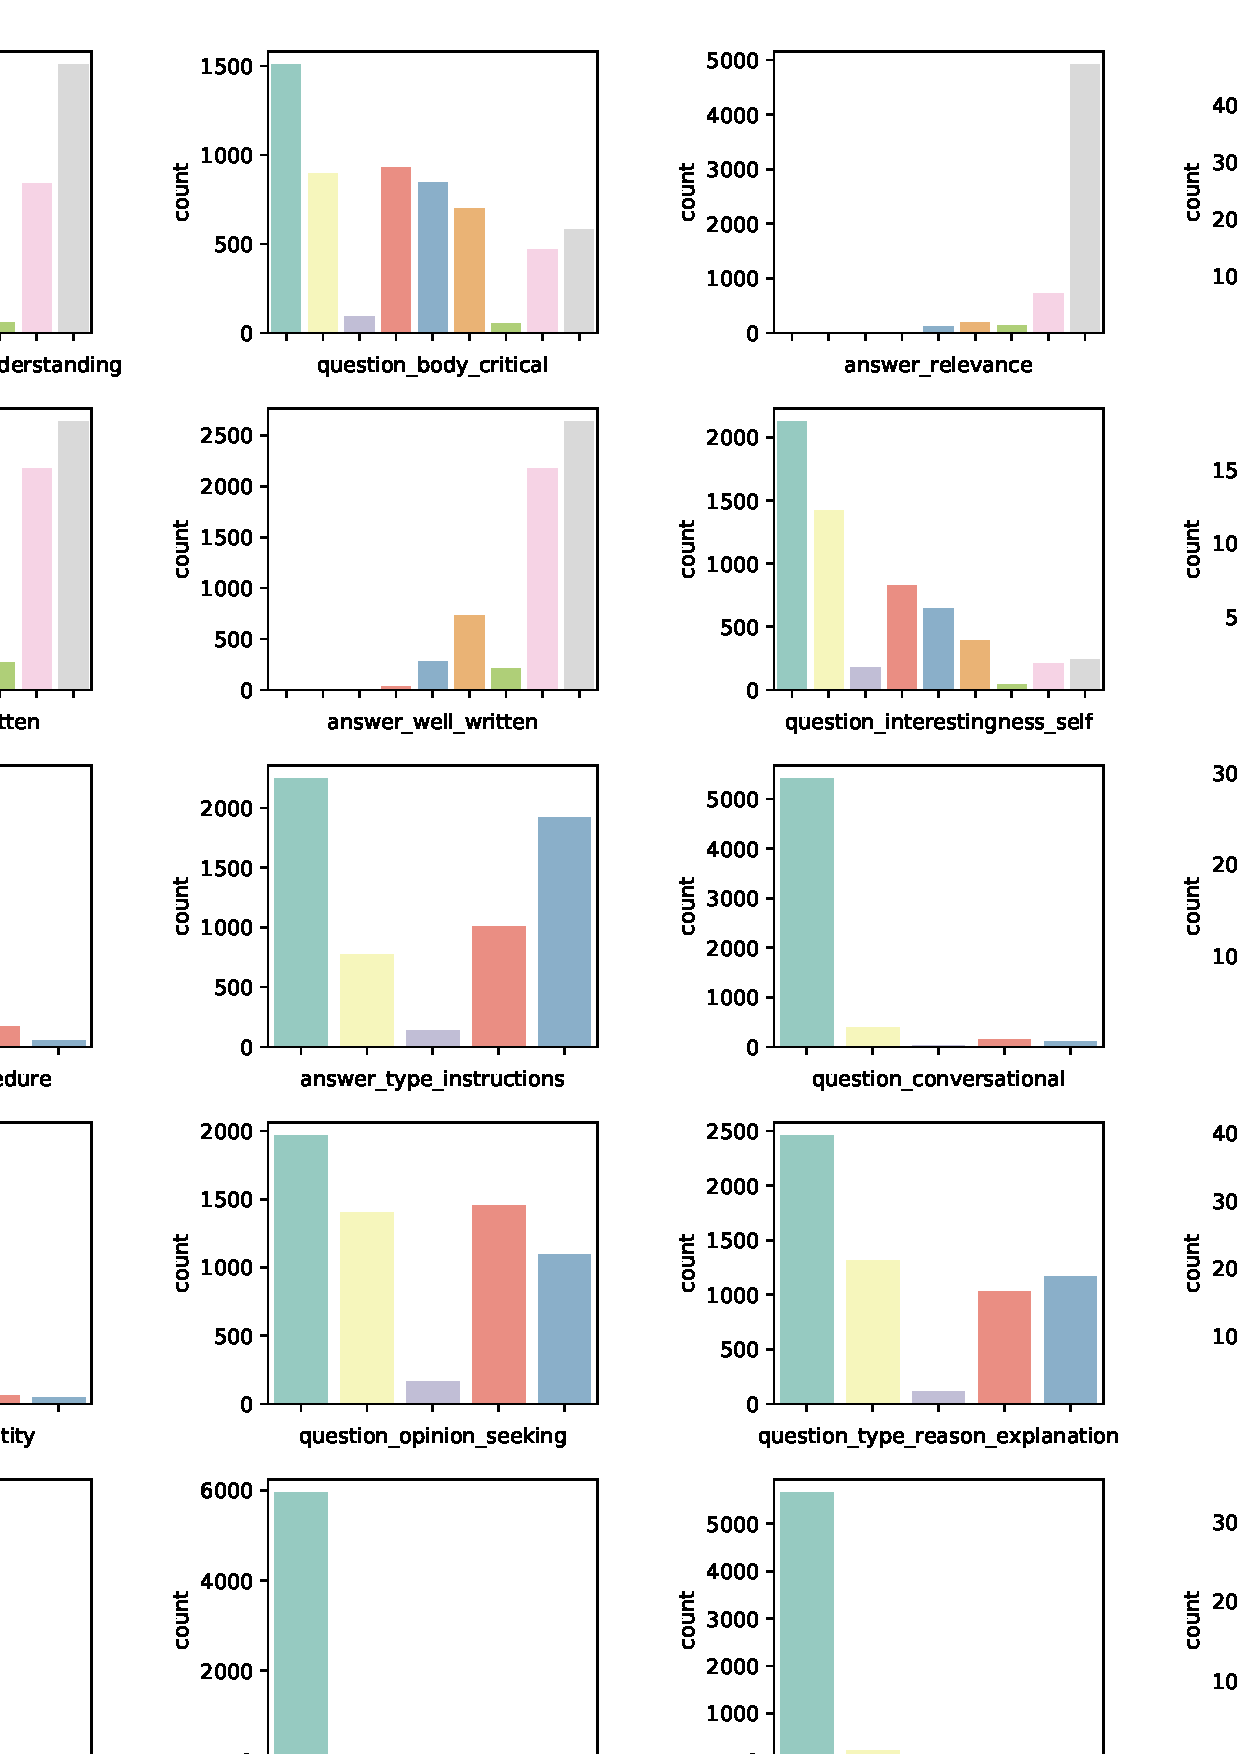
\includegraphics[width=.48\linewidth]{figures/targets.pdf}
    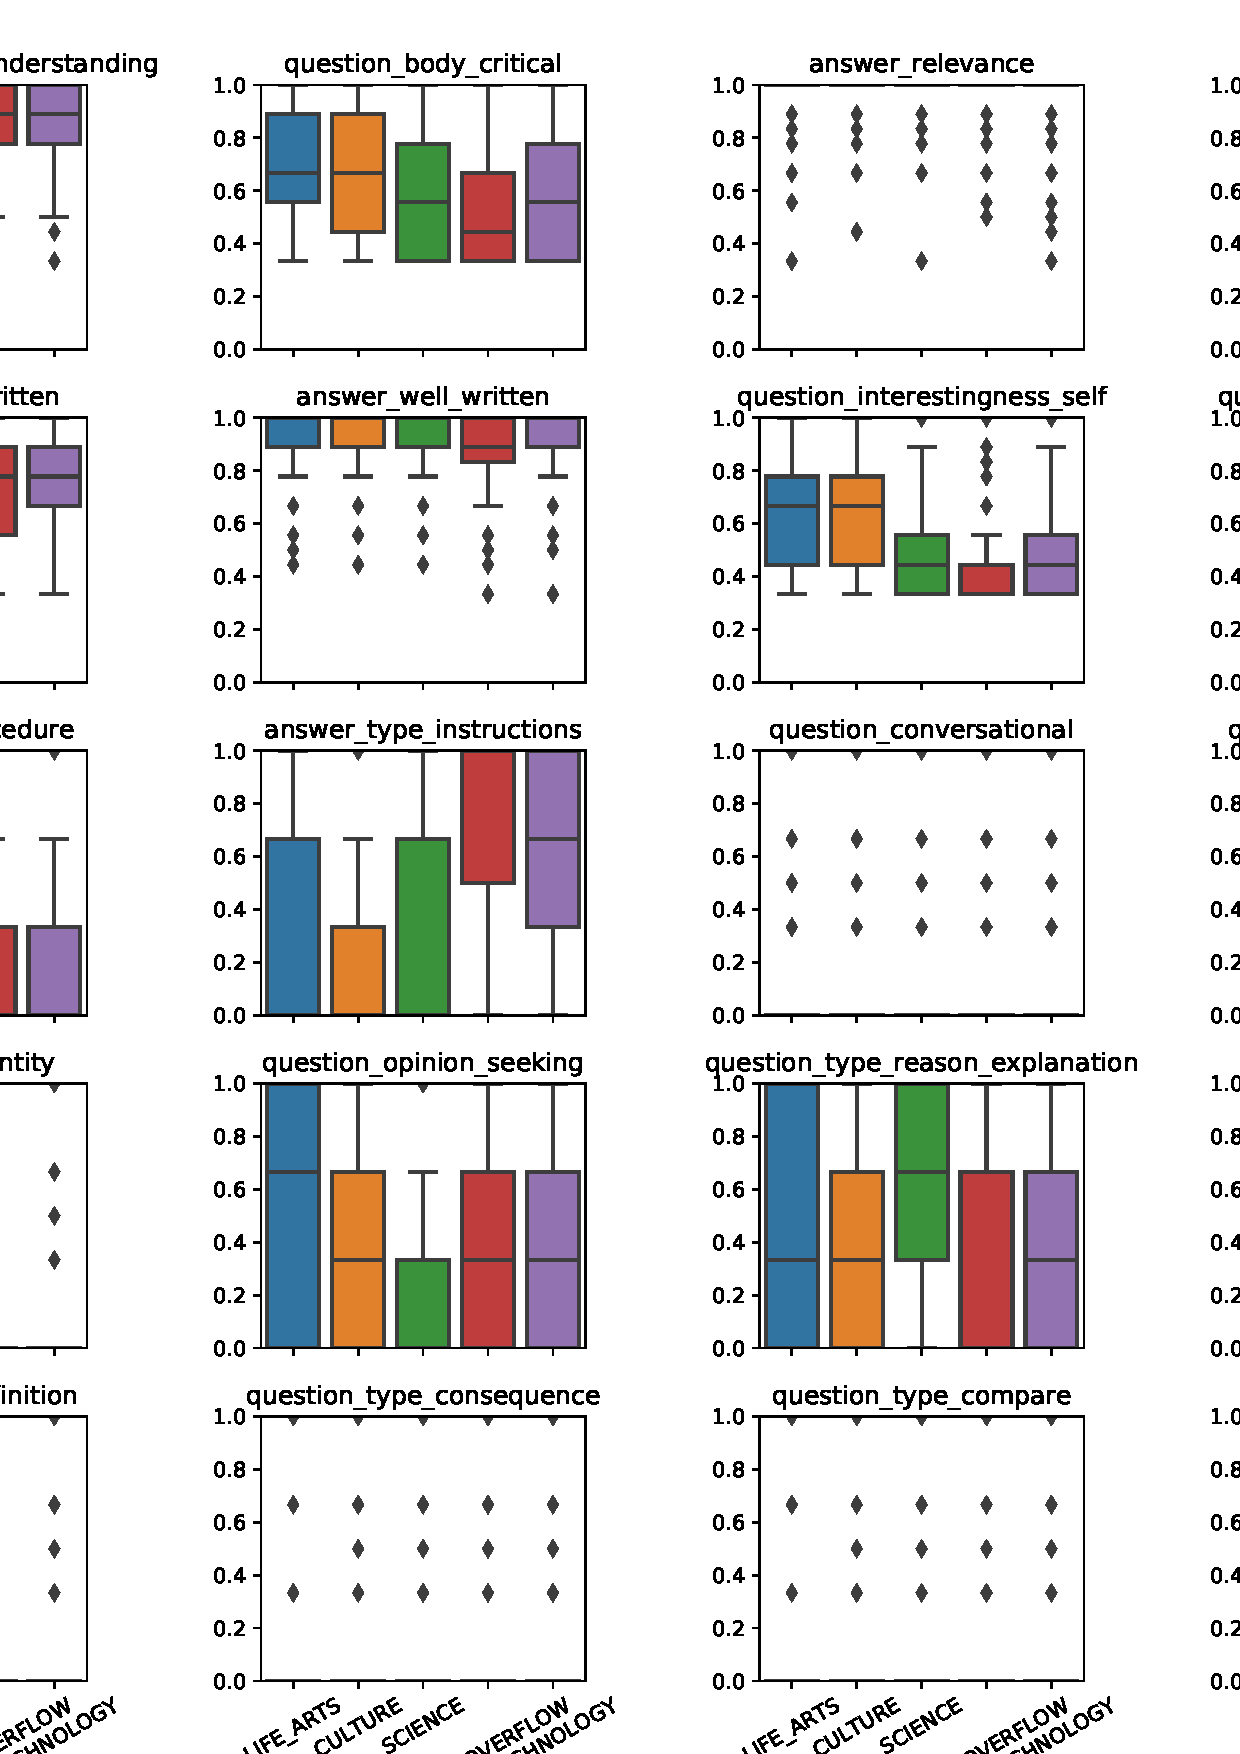
\includegraphics[width=.48\linewidth]{figures/target_category_distribution.pdf}
\end{center}
}
%%%%%%%%%% -------------------------------------------------------------------- %%%%%%%%%%


% SECOND column
\column{0.5}
 %Second column with first block's top edge aligned with with previous column's top.

%%%%%%%%%% -------------------------------------------------------------------- %%%%%%%%%%
\block{Method}{
    \subsection{Embedding}
    The idea of vector semantics is thus to represent a word as a point in some multidimensional semantic space.
    Vectors for representing words are generally called embeddings, because the word is embedded in a particular vector space.
    After convert to embeddings, words with similar meanings are nearby in space.
    
    There are two commonly used vector semantic models. tf-idf and word2vec.
    \subsubsection{Tf-idf}
    The tf-idf algorithm is the product of two terms.
    \begin{itemize}
        \item \textbf{term frequency}:the frequency of the word $t$ in the document $d$. 
        \item \textbf{inverse document frequency}: the inverse of document frequency, which is the number of documents it occurs in.
    \end{itemize}
    \begin{equation}
        tf_{t,d}=count(t,d)
    \end{equation}
    \begin{equation}
        idf_t = \log_{10}{(\frac{N}{df_t})}
    \end{equation}
    Then we get the tf-idf weight value:
    \begin{equation}
        w_{t,d}=tf_{d,f}\times idf_t
    \end{equation}
    The tf-idf vector model represents a target word as a vector with dimensions 
    corresponding to all the words in the vocabulary (length $|V|$, with vocabularies of 20,000 to 50,000).
    The values in each dimension are the frequency with which the target 
    word co-occurs with each neighboring context word, weighted by tf-idf.
    It can also be used to represent a document by the centroid document vector.
    Given $k$ word vectors $w_1, w_2, \dots, w_k$, the centroid document vector $d$ is:
    \begin{equation}
        d = \frac{w_1+w_2+\dots+w_k}{k}
    \end{equation}
    The vector can be used to estimate the similarity between the two word or documents by
    compute $\cos{(d_1, d_2)}$.
    
    \subsubsection{Word2vec}
    The tf-idf vector model represent a word as a sparse, long vector. 
    And it can't capture the words'position information. 
    To do this, the word2vec algorithm is a better choice.
    It also represent words as very short, dense vectors. 
    It turn out that dense vectors work better in every NLP task than sparse vectors.
    
    The skip-gram algorithm is one of two algorithms in a software package called word2vec,
    and so sometimes the algorithm is loosely referred to as word2vec. The intuition of word2vec is that
    given tuple $(t, c)$ of target word $t$ and candidate context word $c$, get whether $c$ is a real context word. (binary classification)
    
    The intuition of skip-gram is:
    \begin{enumerate}
        \item Treat the target word and a neighboring context word as positive examples.
        \item Randomly sample other words in the lexicon to get negative samples.
        \item Use logistic reg to train a classifier to distinguish those two cases.
        \item Use the reg weights as the embeddings.
    \end{enumerate}
}
%%%%%%%%%% -------------------------------------------------------------------- %%%%%%%%%%
% Second column - first block


%%%%%%%%%% -------------------------------------------------------------------- %%%%%%%%%%
\block[titleleft]{Expirement and Analysis}
{


}
%%%%%%%%%% -------------------------------------------------------------------- %%%%%%%%%%


% Second column - second block
%%%%%%%%%% -------------------------------------------------------------------- %%%%%%%%%%
\block[titlewidthscale=1, bodywidthscale=1]{Conclusion}{

}
%%%%%%%%%% -------------------------------------------------------------------- %%%%%%%%%%


% Bottomblock
%%%%%%%%%% -------------------------------------------------------------------- %%%%%%%%%%
\colorlet{notebgcolor}{blue!20}
\colorlet{notefrcolor}{blue!20}
\note[targetoffsetx=8cm, targetoffsety=-4cm, angle=30, rotate=15,
radius=2cm, width=.26\textwidth]{
Acknowledgement
\begin{itemize}
    \item
    International Cooperation Project (Y7Z0511101)
    of IIE,
    Chinese Academy of Sciences
 \end{itemize}
}

%\note[targetoffsetx=8cm, targetoffsety=-10cm,rotate=0,angle=180,radius=8cm,width=.46\textwidth,innersep=.1cm]{
%Acknowledgement
%}

%\block[titlewidthscale=0.9, bodywidthscale=0.9]
%{Acknowledgement}{
%}
%%%%%%%%%% -------------------------------------------------------------------- %%%%%%%%%%

\end{columns}


%%%%%%%%%% -------------------------------------------------------------------- %%%%%%%%%%
%[titleleft, titleoffsetx=2em, titleoffsety=1em, bodyoffsetx=2em,%
%roundedcorners=10, linewidth=0mm, titlewidthscale=0.7,%
%bodywidthscale=0.9, titlecenter]

%\colorlet{noteframecolor}{blue!20}
\colorlet{notebgcolor}{blue!20}
\colorlet{notefrcolor}{blue!20}
\note[targetoffsetx=-13cm, targetoffsety=-12cm,rotate=0,angle=180,radius=8cm,width=.96\textwidth,innersep=.4cm]
{
\begin{minipage}{0.3\linewidth}
\centering
\includegraphics[width=24cm]{logos/tulip-wordmark.eps}
\end{minipage}
\begin{minipage}{0.7\linewidth}
{ \centering
 The $11^{th}$ International Conference on Knowledge Science,
  Engineering and Management (KSEM 2018),
  17-19/08/2018, Changchun, China
}
\end{minipage}
}
%%%%%%%%%% -------------------------------------------------------------------- %%%%%%%%%%


\end{document}

%\endinput
%%
%% End of file `tikzposter-template.tex'.
